
       
       \section{Programação Dinâmica}
\begin{frame}[fragile]
%[fragile, allowframebreaks=0.9]

    \frametitle{Programação Dinâmica -- (PD)}

   \begin{block}{}
     \begin{itemize}
      \item Uma poderosa técnica de programação que  contorna a complexidade de certos problemas
      exponenciais
      
       \pause
       \item O problema \textbf{deve} apresentar uma \textit{\underline{regra de recorrência}}
       
      \pause
      \item A idéia é que todos os cálculos feitos a partir desta \textit{regra de recorrência},
      são consultados e armazenados numa \textit{tabela dinâmica}
      
      \pause
      \item Esta técnica de utilizar uma \textit{tabela dinâmica} nos cálculos intermediários,
      evitando a repetição do que já foi calculado anteriormente, é conhecida como:
      Programação Dinâmica, ou simplesmente: PD

      \pause
      \item Como Picat usa a recursão, na programação em lógica, nada mais
      natural do que esta ter a PD disponível 

       \pause
       \item O comando que cria uma tabela para um determinado predicado é o  \textit{tabling}
 
        \pause
       \item O \textit{tabling}  é um dos elementos fortes do planejador do Picat (módulo \textit{planner})

    \end{itemize}
    
    \end{block}
    
\end{frame}



\begin{frame}[fragile]
%[fragile, allowframebreaks=0.9]

\frametitle{Exemplo de uso da Programação Dinâmica -- (PD)}

Casos particulares do Binômio de Newton são:
\begin{itemize}
  \item  ${\left(x + y\right)}^0 = 1$
  \item  ${\left(x + y\right)}^1 = x + y$
  \item  ${\left(x + y\right)}^2 = x^2 + 2xy + y^2$
  
  \pause
  \item  ${\left(x + y\right)}^2 = x^2y^0 + 2x^1y^1 + x^0y^2$
  \item  ${\left(x + y\right)}^3 = x^3y^0 + 3x^2y^1 + 3x^1y^2 + x^0y^3$
  \item  ${\left(x + y\right)}^4 = x^4y^0 + 4x^3y^1 + 6x^2y^2 + 4x^1y^3 + x^0y^4.$
    \item  .......
    \pause
 \item Como obter estes coeficientes destes polinômios?  

\end{itemize}

    
\end{frame}


\begin{frame}[fragile]
%[fragile, allowframebreaks=0.9]

\frametitle{Exemplo de uso da Programação Dinâmica -- (PD)}

\begin{figure}[!htb]
\centering
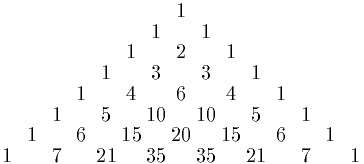
\includegraphics[width=0.70\textwidth, height=0.60\textheight]{figures/pascal_triangle_01.jpg}
%%%prolog/scale=0.47
%\label{fig_nos_estados}
\caption{O triângulo de Pascal}
\end{figure}

   
\end{frame}



\begin{frame}[fragile]
%[fragile, allowframebreaks=0.9]

\frametitle{Exemplo de uso da Programação Dinâmica -- (PD)}

\begin{figure}[!htb]
\centering
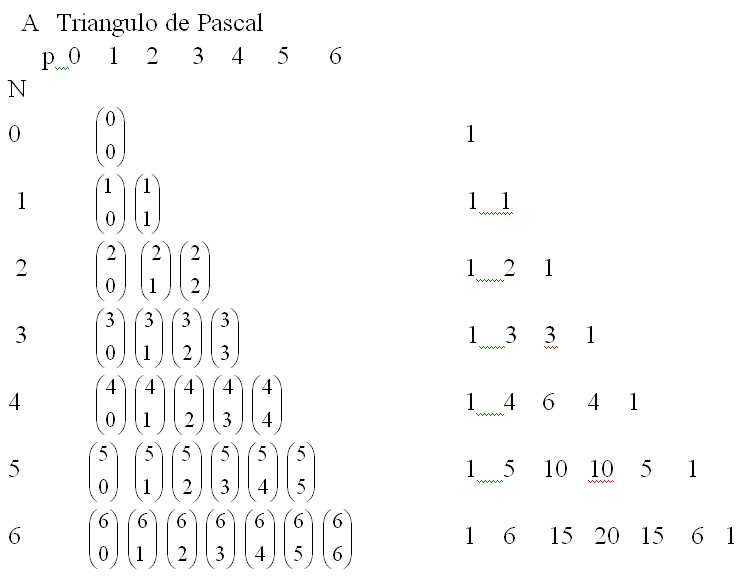
\includegraphics[width=0.850\textwidth, height=0.650\textheight]{figures/pascal_triangle_02.jpg}
%%%prolog/scale=0.47
%\label{fig_nos_estados}
\caption{O triângulo de Pascal -- Coeficientes Binomiais}
\end{figure}

    
\end{frame}



\begin{frame}[fragile]
%[fragile, allowframebreaks=0.9]

\frametitle{Formulação Matemática}

O '''coeficiente binomial''', também chamado de '''número binomial''', de um número n, na classe k, consiste no número de [[Combinação (matemática)|combinações]] de n termos, k a k. O número binomial de um número n, na classe k, pode ser escrito como:

$ {n \choose k}= \frac {n!}{k!(n-k)!}=\frac {n(n-1)(n-2)\cdots(n-k+1)}{k!}$


A relação de Stiffel:

${n-1\choose k-1}+{n-1\choose k}={n\choose k}$
    
 O coeficiente binomial é muito utilizado no Triângulo de Pascal, onde o termo na linha n e coluna k é ${n-1 \choose k-1}$
   
    
\end{frame}




\begin{frame}[fragile] 

\frametitle{Código em Partes}

\begin{verbatim}

import datetime.   %%% para o statistics
import util.


table
c(_, 0) = 1.
c(N, N) = 1.
c(N,K) = c(N-1, K-1) + c(N-1, K).

\end{verbatim}
    
\end{frame}



\begin{frame}[fragile] 

\frametitle{Código em Partes}


\begin{verbatim}
main  ?=>  
    statistics(runtime,_), % faz uma marca do 1o. statistics
    N = 10, %% ateh uns 30 ... são números grandes ... fatorial

     foreach(I in 0  .. N)
        foreach(J in 0  ..  I)
             printf("  %d", c(I,J))
           end,
          printf(" \n"),
      end, 
   
    statistics(runtime, [T_Picat_ON, T_final]),
    T = (T_final) / 1000.0, %%% está em milisegundos
    printf("\n CPU time %f em SEGUNDOS ", T),
    printf("\n OVERALL PICAT CPU time %f em SEGUNDOS ", T_Picat_ON/1000.0),
    
    printf(" \n =========================================\n ")
    %%% , fail descomente para multiplas solucoes
    .
main => printf("\n Para uma solução .... !!!!" ) .
\end{verbatim}

    
\end{frame}


\begin{frame}[fragile]
 \frametitle{Código Completo}

\begin{itemize}
  \item Acompanhar as explicações do código de:\\
\url{https://github.com/claudiosa/CCS/blob/master/picat/coeficiente_binomial_PD.pi}

  \item Confira a execuç\~ao
\end{itemize}
\end{frame}







\begin{frame}[fragile]
%[fragile, allowframebreaks=0.9]

\frametitle{Saída}

\begin{small}
\begin{verbatim}
[ccs@gerzat picat]$ picat coeficiente_binomial_PD.pi 
  1 
  1  1 
  1  2  1 
  1  3  3  1 
  1  4  6  4  1 
  1  5  10  10  5  1 
  1  6  15  20  15  6  1 
  1  7  21  35  35  21  7  1 
  1  8  28  56  70  56  28  8  1 
  1  9  36  84  126  126  84  36  9  1 
  1  10  45  120  210  252  210  120  45  10  1 

 CPU time 0.000000 em SEGUNDOS 
 OVERALL PICAT CPU time 0.009000 em SEGUNDOS  
 =========================================
\end{verbatim}
    
\end{small}
\end{frame}




\begin{frame}[fragile]
\frametitle{Reflexões}


\begin{itemize}
  \item Outros métodos para se resolver estes problemas
  \pause
  \item 
  \pause
   % \pause
  %\item 
\end{itemize}

\end{frame}
